\chapter{Authentication Mechanisms}
\label{cha:authentication_mechanisms}
This chapter explains the concepts and details of the two compared authentication mechanisms.
Only mutual TLS (mTLS) and self-signed JWTs are discussed in more detail since the Trust the Network (TTN) approach is deprecated and should not be used anymore~\cite{dias2020microservices}.
Additionally, the most popular approaches for user-context sharing are discussed since the chosen authentication mechanisms affect how the user-context is shared.

%\begin{figure}
%	\centering
%	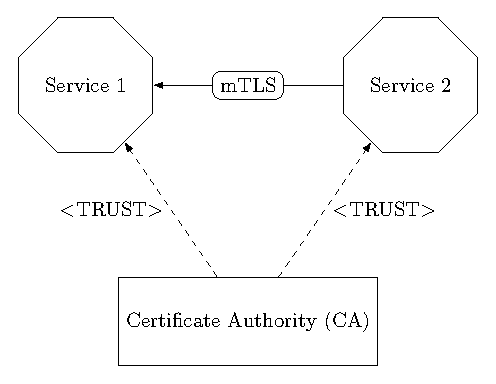
\includegraphics{images/authentication-mechanisms/TikZ_mTLS_base_structure.pdf}
%	\caption{Setup using mTLS for the service-to-service authentication~\cite{dias2020microservices}}
%	\label{fig:auth_mechanisms_mtls}
%\end{figure}

\section{Authentication based on mTLS}
Mutual TLS is the most popular option for service-to-service authentication in microservice deployments~\cite{dias2020microservices}.
Securing the communication with TLS already provides integrity confidentiality and authenticates the server to the client.
Since TLS does not authenticate the client to the server, it is insufficient for service-to-service authentication.
Therefore the efficient and straightforward approach mTLS is used to authenticate the client to the server.

Authentication using mTLS requires a Public Key Infrastructure (PKI~\ref{sec:pki}), same as TLS on the internet.
It is possible to use the already existing PKI of the internet, but this would make the key management much harder and would not bring significant advantages.
Therefore it is good practice to use a self-hosted PKI to have a root of trust within the network~\cite{dias2020microservices}.
%The setup of a microservice deployment using mTLS is shown in figure~\ref{fig:auth_mechanisms_mtls}.

When mTLS is used, the server and the client must provide a valid certificate to create a communication channel.
The issuer of the presented certificates must be trusted by all communicating parties~\cite{dias2020microservices}.
If one communication partner does not have a valid certificate, the communication is neglected.
Therefore each service needs its private key and the corresponding public key.
Additionally, a signed certificate that binds the public key to the certificate's subject is needed.
The certificates of the communication partners are exchanged during the TLS handshake.

This mechanism can also be used to authenticate the end-users of an application.
The term Client Certificate Authentication (CCA) is used for this context~\cite{parsovs2013practical}.
Service-to-service authentication using mTLS is an implementation of CCA, but in this approach, the client is not the end-user, instead, it is another service.

\subsection{Handshake}
\label{sec:tlshandshake_details}
The TLS handshake is used to exchange the certificates of the participants and initialize their connection.
The handshake steps differ between the used algorithms and versions of the TLS protocol.
The following sequence and figure~\ref{fig:tlshandshake} should give an overview about the steps of the TLS handshake using mutual TLS~\cite{parsovs2013practical}:
\begin{enumerate}
	\item The client initializes the connection by sending a \textbf{ClientHello} message to the server.
		The \textbf{ClientHello} message includes a list of supported cipher suites and the randomness.
		The randomness is a combination of random bytes and the current date~\cite{mediumtls}.
	\item The server chooses one cipher suite of the \textbf{ClientHello} message, within the \textbf{ServerHello}.
		Furthermore, the \textbf{ServerHello} contains the server's randomness.
	\item The server sends the \textbf{Certificate} message, containing one or more certificates, that can be used to build the certificate chain.
		The client validates the sent certificates with his truststore.
		If it trusts the sent certificate chain, the handshake is continued.
	\item The server sends the \textbf{CertificateRequest} message, providing a list of all CAs he trusts.
		The client can use this list to choose the correct certificate he has to present for the Client Certificate Authentication.
	\item The server sends the \textbf{ServerHelloDone} message, signalizing that the server finished his Hello message.
	\item The client responds with his \textbf{Certificate} message, which is similar to the servers \textbf{Certificate} message, but contains the client's certificate chain.
	\item The client generates a random value, the pre-master secret, that is later used to derive symmetric keys for the cryptographic operations defined in the cipher suite.
		The pre-master secret is encrypted using the server's public key.
		Therefore, only the owner of the corresponding private key, the server, can decrypt this message.
		In the end, the encrypted pre-master secret is transferred to the server within the \textbf{ClientKeyExchange} message.
	\item The client has to prove that he owns the corresponding private key of the certificate he sent.
		Therefore he has to encrypt the hash of all previous messages with his private key.
		This encrypted hash is then sent to the server within the \textbf{CertificateVerify} message.
		The server can decrypt the hash and can calculate it on his own to check whether the decrypted hash is correct or not.
	\item The client sends a \textbf{ChangeCipherSpec} message to signal the server that all following messages will be protected with the protection mechanisms defined in the cipher suite.
	\item The last message of the handshake, the \textbf{Finished} message contains an encrypted has of all previous messages.
	%\item[11-12] Same as steps 9-10 but from the server.
	\item Same as step 9, but from the server.
	\item Same as step 10, but from the server.
\end{enumerate}
The handshake would have almost the same steps when mTLS is not used.
Only the \textbf{CertificateRequest} message of the sever and the \textbf{Certificate} message and the \textbf{CertificateVerify} message of the client are unique for mTLS~\cite{parsovs2013practical}.
%One special case of the handshake is that the client responds to the \textbf{CertificateRequest} with an empty \textbf{Certificate} message.
%Depending on the configuration of the server, the connection without a certificate can be allowed or neglected~\cite{parsovs2013practical}.

\newcommand{\newthreadShift}[4][gray!30]{
  \newinst[#4]{#2}{#3}
  \stepcounter{threadnum}
  \node[below of=inst\theinstnum,node distance=0.8cm] (thread\thethreadnum) {};
  \tikzstyle{threadcolor\thethreadnum}=[fill=#1]
  \tikzstyle{instcolor#2}=[fill=#1]
}

\begin{figure}
	\centering
	\begin{sequencediagram}
		\renewcommand\unitfactor{0.8}
		\newthread{A}{:Client}{}
		\newthreadShift{B}{Server}{11cm}
		%\newinst[11]{B}{:Server}{}
		\begin{messcall}{A}{ClientHello$^1$}{B}{}
			\mess{B}{ServerHello$^2$, Certificates$^3$, CertificateRequest$^4$, ServerHelloDone$^5$}{A}
			\mess{A}{Certificate$^6$, ClientKeyExchange$^7$, CertificateVerify$^8$}{B}
			\mess{B}{ChangeCipherSpec$^9$, Finished$^{10}$}{A}
			\mess{A}{ChangeCipherSpec$^{11}$, Finished$^{12}$}{B}
		\end{messcall}
	\end{sequencediagram}
	\caption{TLS handshake using mTLS~\cite{parsovs2013practical}}
	\label{fig:tlshandshake}
\end{figure}

%\begin{figure}
%	\centering
%	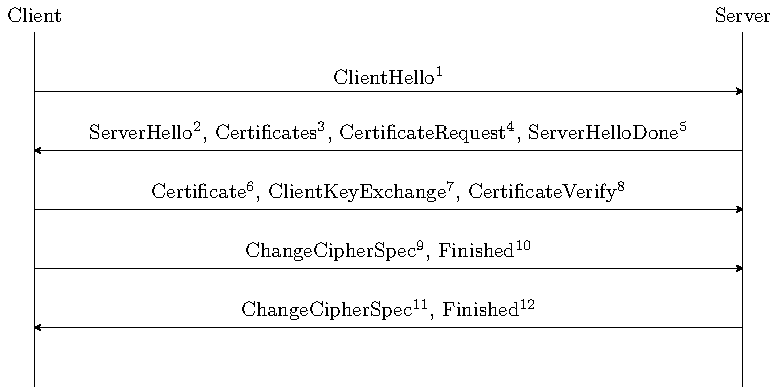
\includegraphics{authentication-mechanisms/TikZ_handshake.pdf}
%	\caption{TLS handshake using mTLS~\cite{parsovs2013practical}}
%	\label{fig:tlshandshake}
%\end{figure}

\subsection{Passing the end user context} \label{sec:mtls_end_user_context}
In some cases, not only the identity of the microservice but also the identity of the end-user is relevant.
Then, the microservices have to pass the end-user context when they consume the logic of other microservices.
The most popular approach for passing the end-user context are JSON Web Tokens.
The JWTs can be embedded within the HTTP Request body or using URL parameters.
This approach can be implemented in multiple ways~\cite{dias2020microservices}.

\begin{figure}[H]
	\centering
	\begin{sequencediagram}
		\newthread{client}{:Client}{}
		\newinst[1]{gateway}{:API Gateway}{}
		\newinst[1]{sts}{:STS}{}
		\newinst[1]{s1}{:Service1}{}
		\newinst[1]{s2}{:Service2}{}

		\begin{call}{client}{access token}{gateway}{response}
			\begin{call}{gateway}{access token}{sts}{JWT$^1$}
			\end{call}
			\begin{call}{gateway}{JWT$^1$}{s1}{response}
				\begin{call}{s1}{JWT$^1$}{s2}{response}
				\end{call}
			\end{call}
		\end{call}
	\end{sequencediagram}
	\caption{Identity propagation using the same JWT for each request~\cite{dias2020microservices}}
	\label{fig:mtls_id_1}
\end{figure}

\newpage
Generally, the user has to obtain an access token from any token service.
This token could be an OAuth2, OpenID Connect, or any other token.
Then the user has to embed his token within the Authorization header of each request.
The token is validated by a Security Token Service (STS).
If the token is valid, the STS returns a JWT that can then be used to consume other services.
When one microservice uses the API of another microservice, he embeds the received JWT within the request.
If this microservice has to use the API of another microservice, he also passes the same token to the next microservice~\cite{dias2020microservices}.
The workflow of this approach is shown in figure~\ref{fig:mtls_id_1}


%\begin{figure}
%	\centering
%	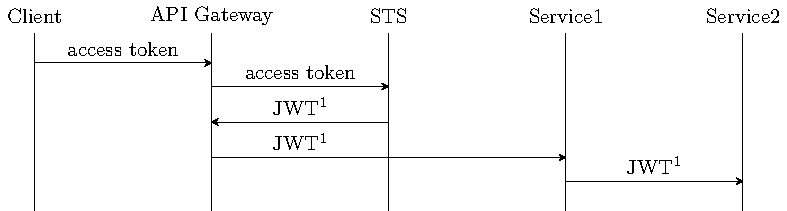
\includegraphics{images/authentication-mechanisms/TikZ_jwt_identity_1.pdf}
%	\caption{Use the same JWT for each request~\cite{dias2020microservices}}
%	\label{fig:mtls_id_1}
%\end{figure}

Another approach is that the STS is used to generate a new token for each request, as shown in figure~\ref{fig:mtls_id_2}.
When the STS generates a new token for each request, he fully knows all performed requests.
Therefore the STS could implement further authorization logic~\cite{dias2020microservices}.
Nevertheless, the frequent calls could result in an additional workload for the STS and decrease the system's performance.

\begin{figure}
	\centering
	\begin{sequencediagram}
		\newthread{client}{:Client}{}
		\newinst[1]{gateway}{:API Gateway}{}
		\newinst[1]{sts}{:STS}{}
		\newinst[1]{s1}{:Service1}{}
		\newinst[1]{s2}{:Service2}{}

		\begin{call}{client}{access token}{gateway}{response}
			\begin{call}{gateway}{access token}{sts}{JWT$^1$}
			\end{call}
			\begin{call}{gateway}{JWT$^1$}{s1}{response}
				\begin{call}{s1}{JWT$^1$}{sts}{JWT$^2$}
				\end{call}
				\begin{call}{s1}{JWT$^2$}{s2}{response}
				\end{call}
			\end{call}
		\end{call}
	\end{sequencediagram}
	\caption{Identity propagation using a new JWT for each request~\cite{dias2020microservices}}
	\label{fig:mtls_id_2}
\end{figure}

%\begin{figure}[H]
%	\centering
%	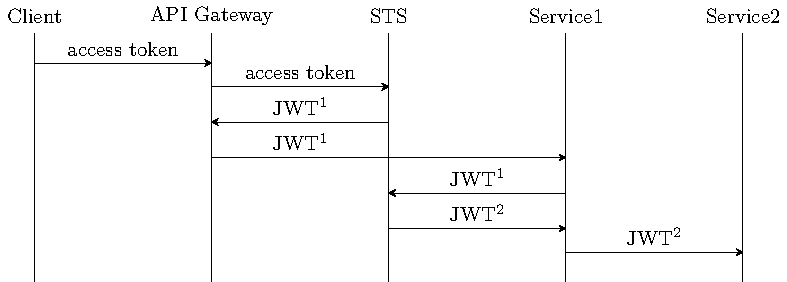
\includegraphics{images/authentication-mechanisms/TikZ_jwt_identity_2.pdf}
%	\caption{Generate new JWT for each request~\cite{dias2020microservices}}
%	\label{fig:mtls_id_2}
%\end{figure}

Both approaches result in some overhead, especially the approach creating a new JWT for each request.
Additionally, when the microservices are located in different trust domains, those approaches can get very complicated since a microservice only trusts the STS within its trust domain~\cite{dias2020microservices}.
The problem with JWTs is that they can be stolen and used by intruders.
Therefore it is necessary to provide mutual authentication, confidentiality, and integrity when JWTs are used to share the user context.

\subsection{Conclusion}
mTLS is an efficient mechanism to implement service-to-service authentication.
Since the communication between the services is usually secured using TLS, the configuration of mTLS does not cause much overhead, and no new technologies are necessary~\cite{dias2020microservices}.

A crucial advantage of the TLS handshake is that the private keys are never exchanged, and the session keys are always different due to the usage of the randomness.
% Unclear antecedent
Therefore, even if an intruder can get the session key of a communication channel, he cannot use this key for another session.
Furthermore, it is not possible to retrieve any information about the private key of the communication partners with the knowledge of the session key.
% Unclear antecedent
This shows how secure mTLS is, even for advanced attacks~\cite{parsovs2013practical}.

From the developer's perspective, mTLS does not require much implementation logic.
The service that acts as the server has to be configured to use client certificate authentication.
%Possilbly wordy sentence
Depending on the used technologies, this is usually done by setting a few configuration parameters in the code or directly on the webserver.
The service that acts as the client has to be configured to send his certificate during the TLS handshake.
Most HTTP Client libraries support simply attaching the certificate to each HTTP request.
Nevertheless, the developers do not have to implement much logic resulting in the problem that they do not have much control over the system.
The developers have to rely on the implementation of the webserver developers.
When a web server has security-related bugs, the microservice developers can not solve them independently.
For example, the apache webserver, one of the most popular webservers, had many issues in combination with CCA.
Arnis Parsovs~\cite{parsovs2013practical} researched the problems of the apache webserver and gave an extensive guide on how to circumvent all bugs when CCA is configured.

Key management is the biggest challenge of mTLS, it was described in more detail in chapter~\ref{sec:key_management}.
It is responsible for key provisioning, revocation, rotation, and more management tasks.
Usually, key management requires a self-hosted PKI for the deployment.
For small applications, the key management can be kept very simple.
As soon as the deployment grows and many services run simultaneously, automation tools are required.
Therefore the management overhead of mTLS is much more complicated to handle than the implementation of mTLS itself~\cite{dias2020microservices}.

The previously mentioned challenges and motivation result in the conclusion that mTLS is a beneficial and efficient approach when the developers do not require to fully control each aspect of the authentication.
Especially when the end-user context has to be shared among the services, mTLS might not be the most efficient solution.
mTLS may not be the ultimate tool for all security challenges.
Still, when the requirement is service-to-service authentication, mTLS does its job, and it does it well.
% Unclear antecedent
Therefore mTLS is the most popular approach for service-to-service authentication.

\section{Authentication based on self-signed JWTs}
Self-signed JWTs can be used to provide mutual authentication for service-to-service communication.
Same as mTLS, it is based on asymmetric cryptography, and each service needs to own a key pair.
The main idea is that the sender creates a JWT signed with his private key.
The receiving service can then check the signature of the JWT with the public key of the service that sent the request.
The signed JWT is transferred within the Authorization header of the HTTP request~\cite{dias2020microservices}.
%This workflow is visualized in figure~\ref{fig:auth_mechanisms_jwt}.
Since the JWT does not have any fixed structure, it is possible to embed contextual data like the user context as claims within the JWT.
Therefore parameters and information about the user do not have to be passed within the body or as URL parameters~\cite{dias2020microservices}.

%\begin{figure}
%	\centering
%	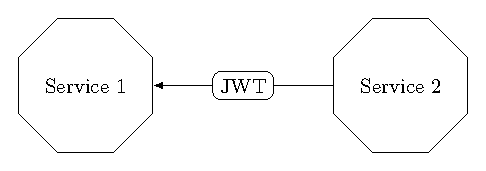
\includegraphics{images/authentication-mechanisms/TikZ_jwt_base_structure.pdf}
%	\caption{Setup using self signed JWTs for the service-to-service authentication~\cite{dias2020microservices}}
%	\label{fig:auth_mechanisms_jwt}
%\end{figure}

The usage of self-signed JWTs does not provide confidentiality for the communication among the services.
Therefore TLS should be used to provide confidentiality for service-to-service communication.
Since the mechanism is not dependent on TLS, it is possible to use other mechanisms instead of TLS.
For example, JSON Web Encryption or any other encryption mechanism can be used, but usually, it does not make sense to get rid of TLS~\cite{dias2020microservices}.
When TLS is not used, other mechanisms have to authenticate the server to the client.

The usage of self-signed JWTs additionally provides nonrepudiation.
% Possibly wordy sentence
Therefore each action is bound to the service that created the JWT, and the service can not repudiate that the JWT was created by him~\cite{dias2020microservices}.
Whenever nonrepudiation is a requirement of the system, self-signed JWTs are the superior authentication mechanism.

\subsection{Nonrepudiation}
Digital signatures can be used to achieve nonrepudiation cryptographically.
Nonrepudiation binds the actions performed by a service to the service or API Gateway who initiated the action.
In general, the recipient of a message is provided with proof of the message's origin.
Therefore the recipient is protected against situations when a sender denies that he sent a message~\cite{wu20131200}.

Nonrepudability and authentication are very similar.
Authentication is about convincing the other party that an event is valid.
With nonrepudiation, it is even possible to prove the truth of an event to a third party~\cite{wu20131200}.

A practical example that requires nonrepudiation is an online shop.
Assuming that the shop has an \textbf{OrderService} and a \textbf{PaymentService}.
When the payment is accomplished using the functionalities of the \textbf{PaymentService}, it has to signalize the \textbf{OrderService} that the order was paid.
Therefore the \textbf{PaymentService} would send a request to the \textbf{OrderService} containing a JWT signed using the private key of the \textbf{PaymentService}.
When the \textbf{OrderService} stores the JWT and the request, it can always prove that the request was originated by the \textbf{PaymentService}.
No other service could have created the JWT because only the \textbf{PaymentService} can create a valid signature for his public key.

\subsection{Passing the end-user context}
The mechanisms of how the end-user context is passed between the services are similar to the mechanisms explained in~\ref{sec:mtls_end_user_context}.
The big difference is how the JWT is transferred among the services.
% Possibly wordy sentence
With mTLS, the JWT was embedded within the body or as a URL parameter, with self-signed JWTs, it can be embedded within the JWT that already has to be transferred.
% Unclear antecedent
This is done by appending a nested JWT within the claims of the self-signed JWT.
The signature of the JWT, which is used for authentication, can still be verified by using the service's public key.
The signature of the nested JWT is verified using the public key of the STS.
% Unclear antecedent
This means the JWT is carried in a way that can not be forged.
Therefore it is better to use self-signed JWTs for authentication when the end-user context is relevant in many situations~\cite{dias2020microservices}.

\subsection{Conclusion}
Service-to-service authentication using self-signed JWTs is not only a mechanism for authentication. It additionally provides nonrepudiation and makes sharing the user context more convenient. 
Otherwise, the implementation of self-signed JWTs is more challenging than the implementation of mTLS.
It is insufficient to configure the webserver correctly and append a certificate to each request.
Every service has to know how to encode and decode JWTs.
Furthermore, all received JWTs must be stored for an adequate timespan to achieve nonrepudiation, requiring additional database storage.

One significant advantage of self-signed JWTs is that the developers can vary the implementation depending on their needs.
For example, the developers can vary the technology used to provide confidentiality. 
Even if this might not be necessary in most cases, the possibility can be an advantage~\cite{dias2020microservices}.
Furthermore, the developers can define additional parameters that must be provided within the transferred JWTs.
This freedom of choice is not guaranteed with mTLS because it is a strictly defined protocol with very few configuration options.

Sadly the biggest challenge of mTLS, key management, can not be avoided using self-signed JWTs, because it also requires each service to have its key pair.
Therefore a PKI is required for both mechanisms.
But, the key management can be simplified since it is unnecessary to have a CA responsible for signing each certificate.
Still, it makes sense to have one superior authority regarding the webserver setup, that is, the root of trust and whose chained certificates are trusted.

As a result, self-signed JWTs are the preferred authentication mechanism when the target is to achieve nonrepudiation or when the system is very dependent on sharing the user context.
Nevertheless, this leads to additional implementation overhead and requires developers specialized in security-related systems.
evertheless, this leads to additional implementation overhead and requires developers specialized in security-related systems.
